\chapter{非线性演化方程三种波解的构造算法及其机械化实现}\label{ch02}
Hirota 方法是构造非线性微分方程精确解的一种有效方法, 基于 Hirota 方法可构造非线性演化方程的孤子解\D 呼吸子解和 lump 解等. 本文在\refchp{ch01}中介绍了多个基于 Hirota 方法的机械化工作, 但是这些工作主要存在以下问题:
\begin{inparaenum}[(1)]
\item \red{主要用于求多孤子解, 对于其它类型的解暂无机械化实现}.
\item 因为 Hirota 方法的局限性, 这些工作只能保证在求解可积方程时是有效的, \red{对于不可积的方程往往不能构造出满足原方程的$n$孤子解}. 
\item 对于方程的变换, 有的需要人工输入, 有的只考虑了对数变换. 
\end{inparaenum}

针对以上\red{问题}, 本章基于\Painleve{}展开法\D 简单Hirota方法等, 发展出了构造非线性演化方程三种波解的机械化算法, 并研发了相应的软件. \red{特别地, 我们完善了计算$n$孤子解的公式, 给出了一种参数约束条件, 使得$n$孤子解的公式对不可积方程也有效.}

\section{\Painleve{}展开法}

Hirota 方法中第一个关键步骤就是找到一个合适的变换. 常见的变换有对数变换\D 有理变换\D 复合函数变换等.  此外, \Painleve{}展开法也是确定变换的一个有效方法. \Painleve{}展开法所确定的变换是一个\Painleve{}截断展开(Truncated \Painleve{} Expansion, 简称TPE). 该方法由Conte\cite{conte1989invariant}提出, 后经Pickering\cite{pickering1993new}和楼森岳\cite{lou1998extended}完善, 能够用于求 NLEE 的精确解.

事实上, 已有多个关于\Painleve{}展开法的机械化实现. 如 Rand\cite{rand1986odepainleve}\D Ranner\cite{renner1992constructive}\D Scheen\cite{scheen1997implementation}\D Hereman\cite{hereman1989painleve,hereman1998algorithmic}\D Baldwin\cite{baldwin2004symbolic,baldwin2006symbolic}\D 徐桂琼\cite{xu2004symbolic,xu2005pdeptest,xuPHD}和赵银龙\cite{zhaoMST}等人都对\Painleve{}展开法进行了实现. 他们的实现除了求解 TPE 以外, 还关注共振点的分析, 主要用于分析方程的可积性. 因为 TPE 的求解不是这些工作的主要内容, 所以他们并没有深入讨论 TPE 的求解算法. 于是, 为了更加全面地处理求解中可能出现的各种情况, 本文提出了一个递归算法来求解 TPE. 同时, 本文还结合 $n$阶展开方法完善了 TPE 的阶数分析, 并开发了相应的软件包 PExpand. 

\Painleve{}展开法的具体步骤如下. 

对于一个$n+1$维的未知函数$u=u(x_1,\cdots,x_n,t)$, 关于它的 NLEE 是一个关于$u$及其导数的多项式方程, 即
\begin{equation}
    U(u,u\up{1},u\up{2},u\up{3}\cdots)=0, \label{oeq}
\end{equation}
其中$u\up{k}~(k=1,2,3,\cdots)$表示所有的$k$阶导数. 例如, $u\up{1}=\bbrace{u_t,u_{x_1},\cdots,u_{x_n}}$, 以及$u\up{2}=\bbrace{u_{t,x_1},\cdots,u_{t,x_n},u_{x_1,x_2},\cdots}$.

假设原方程存在TPE
\begin{equation}
    u=\sum_{k=1}^{m}{\frac{u_k(x_1,\cdots,x_n,t)}{f^{m-k+1}}},  \label{tr}
\end{equation}
其中$f=f(x_1,\cdots,x_n,t)$, 而$m$的值可以通过通过齐次平衡原则来确定. 

因为
\begin{equation}
    \DIF{x}\frac{1}{f}=-\frac{f_x}{f^2},
\end{equation}
所以\refeqn{tr}的导数仍然是关于$1/f$的多项式, 且求导一次则次数加一. 可分析方程各项代入\refeqn{tr}后关于$1/f$的次数来确定$m$的值.

例如, 对KdV方程\CITEaaKdV{}
\begin{equation}
    u_t+\alpha uu_x+u_{xxx}=0,
\end{equation}
可得其各项次数为$\mbrace{m+1,2m+1,m+3}$. 在齐次平衡原则中, 需要平衡其线性最高次项和非线性最高次项的阶数, 即$m+3=2m+1$, 得$m=2$. 在本文的\refchp{ch04}中, 我们将介绍如何使用本文提出$n$阶展开方法来更加全面地分析平衡的情况. 

一旦确定了$m$的值, 就将\refeqn{tr}代入\refeqn{oeq}, 令$1/f$不同幂次的系数的系数为零就能依次求解$u_1,u_2,\cdots,u_m$. 事实上, 这个求解过程是可以简化的. 首先, 根据 
\begin{equation}
    \DIF{x}\frac{u_k}{f}=\frac{\DIF{x}u_k}{f}-\frac{u_kf_x}{f^2}
\end{equation} 
可以发现, 在最高次项中不会出现 $u_k$ 的导数. 代数方程的求解比微分方程的求解更加简单, 我们选择先从$1/f$的最高次项中求解$u_1$, 然后将$u_1$代入下一项继续求解$u_2$, 以此类推. 按照这种方法求解$u_k$可能碰到以下问题: 
\begin{compactenum}[(1)]
\item $u_k$多解, 则需要遍历每个解继续代入求解$u_{k+1},u_{k+2},\cdots$.
\item 代入$u_1,\cdots,u_k$的解之后, 当前项的系数为零, 则需要继续代入下一项才能求解$u_{k+1}$. 
\end{compactenum}
为了解决上述问题, 本文设计了如\refalg{rpsolve}所示的递归求解算法. 

\begin{algorithm}[t]
\caption{TwSolver: \Painleve{}展开法中的递归求解算法}\label{rpsolve}
\KwIn{当前解集$s$, 当前需要求解的方程编号$n$, 全部方程$eqs$, 全部变量$vrs$.}
\KwOut{$eqs$关于$vrs$的所有截断解.}
\Fn{\rm $\cd{rpsolve}(s,n,eqs,vrs)$}{
    \If{$s=\emptyset$}{
        \Return{\rm $\cd{rpsolve}([~],n,eqs,vrs)$}\tcp*[r]{初始调用}
    }
    \If{$type(s)=set$}{
        \Return{\rm $\bigcup\limits_{t\in s}{\cd{rpsolve}(t,n,eqs,vrs)}$}\tcp*[r]{对解集中的每个解进行遍历}
    }
    \If{$s.length=vrs.length$}{
        \Return{${s}$}\tcp*[r]{所有变量求解完成则返回当前解}
    }
    \If{$n>eqs.length$}{
        \Return{$\emptyset$}\tcp*[r]{所有方程都已经求解时还有变量未解则表示无解}
    }
    $eq\gets eval(eqs[n],s)$\tcp*[r]{将当前解代入后获得新方程}
    \If{$eq=0$}{
        \Return{\rm $\cd{rpsolve}(s,n+1,eqs,vrs)$}\tcp*[r]{当前方程恒成立则代入下一个方程求解}
    }
    $r\gets solve(eq,vrs[s.length+1])$\tcp*[r]{求解当前变量}
    \If{$r=\emptyset$}{
        \Return{$\emptyset$}\tcp*[r]{当前变量无解, 前面的解也无效, 整体返回空集}
    }
    $ns\gets \bigcup\limits_{t\in r}{s.append(t)}$\tcp*[r]{当前变量解集中的每个解添加到已有的解中构成新的解集}
    \Return{\rm $\cd{rpsolve}(ns,n+1,eqs,vrs)$}\tcp*[r]{继续求解下一个变量}
}
\end{algorithm}

在\refalg{rpsolve}中, 我们定义了\cd{rpsolve}函数. 在该函数中, 
\begin{compactitem}[\textbullet]
\item \cd{eqs} 是需要求解的方程组, 即 $1/f$ 的各项系数, 且按次数从高到低排列.
\item \cd{n} 表示当前需要求解方程 \cd{eqs[n]}. 
\item \cd{vrs} 是需要求解的变量, 即$u_1,\cdots,u_m$.
\item \cd{s} 表示当前已经获得的解. 当\cd{s}是一个集合时, 表示它是多个解的集合; 当\cd{s}是一个列表时, 表示它是一个解. 例如, 当$s=\bbrace{\mbrace{f_1,f_2},\mbrace{f_3,f_4}}$时, 表示目前已经解得两组解: $\bbrace{u_1=f_1, u_2=f_2}$ 和 $\bbrace{u_1=f_3, u_2=f_4}$. 将这个参数传递给 \cd{rpsolve}, 它将会分别以 $s=[f_1,f_2]$ 和 $s=[f_3,f_4]$ 为参数调用自身, 并返回结果的并集. 当输入参数是 $s=[f_1,f_2]$ 时, \cd{rpsolve} 会将把 $\bbrace{u_1=f_1,u_2=f_2}$ 代入到 \cd{eqs[n]} 中求解 $u_3$. 
\item 最后, 调用\cd{rpsolve(\{\},eqs,vrs)}就能求得所有解.
\end{compactitem}

此外, 因为求解过程中既需要求解代数方程, 也可能求解微分方程, 故采用 Maple 中的 \cd{PDEtools:-Solve} 函数进行求解. 

基于\refalg{rpsolve}完成$u_1,\cdots,u_k$的求解之后, 选择一组解, 将其代入到\refeqn{tw}中, 就能得到一个TPE
\begin{equation}
u=\sum_{k=1}^m{\frac{u_k}{f^{m-k+1}}}.    
\end{equation}

事实上, TPE可以看作是对数变换的推广. 例如, 对数变换
\begin{equation}
u=R[\ln(f)]_x=R\frac{f_x}{f} \text{~~~和~~~} u=R[\ln(f)]_{xx}=R\sbrace{\frac{f_{xx}}{f}-\frac{f_x^2}{f^2}}
\end{equation}
都满足TPE的形式.

最后, 将得到的变换代入\refeqn{oeq}并取分子, 就可以得到关于$f$及其导数的方程, 即
\begin{equation}
    F(f,f\up{1},f\up{2},f\up{3}\cdots)=0. \label{feq}
\end{equation}

\section{简单 Hirota 方法与孤子解}
在利用\Painleve{}展开法确定变换之后, 可通过简单 Hirota 方法来构造NLEE的孤子解. 

设$f$为行波变量$\xi$的函数, 其中
\begin{equation}
    \xi=p_1\sbrace{x_1+p_2x_2+\cdots+p_nx_n+\omega t}+p_{n+1}. \label{tw}
\end{equation}
这里, $PL=\mbrace{p_1,p_2,\cdots,p_{n+1}}$ 是参数列表. 例如, 当$PL=[k,p,q,c]$时, 
\begin{equation}
    \xi=k(x+py+qz+\omega t)+c.
\end{equation}
将
\begin{equation}
    f=1+\exp\sbrace{\xi} \label{1-soliton}
\end{equation}
代入\refeqnn{feq}后可以求出色散关系$\omega$. 

对于一个包含$p_i~(i=1,\cdots,n+1)$的表达式$e$, 我们定义\emph{下标映射函数}
\begin{equation}
    S(e,k;\PS): \left\{\begin{array}{ll}
        p_i \rightarrow p_{i,k} & i \in \PS, \\ 
        p_i \rightarrow p_i & i \not\in \PS,
    \end{array}\right.
\end{equation}
其中 $\PS$ 是\emph{参数下标集合}, 且有 
\begin{equation}
    \PS\subseteq  \ALLP=\bbrace{1,2,\cdots,n,n+1}.
\end{equation}
在本文中, $\subseteq$ 表示子集, $\subsetneq$ 表示真子集. 

将
\begin{equation}
    f=1+\exp\sbrace{\xi_i}+\exp\sbrace{\xi_j}+h_{i,j}\exp\sbrace{\xi_i+\xi_j} \label{hij}
\end{equation}
代入\refeqnn{feq}后, 可以求出相互作用系数$h_{i,j}$. 这里, $\xi_i=S(\xi,i;\PS)$, $\xi_j=S(\xi,j;\PS)$.

当$\omega$和$h_{i,j}$都有解时, 就可以计算方程的多孤子解. 否则, 算法结束. 我们称$\omega$和$h_{i,j}$都有解的方程是\emph{可解的}; 否则, 方程是\emph{不可解的}.

需要注意的是, $\PS$在我们的算法中是非常关键的. $\PS= \ALLP$表示算法会根据孤子解的公式生成没有参数约束的解. 本文引入$\PS$的理由如下: 
\begin{compactenum}[1. ]
\item 对于一些不可积的方程, 取$\PS= \ALLP$会得到\emph{\FalseSol{}}(不满足原方程的解). 但是, 取$\PS\subsetneq  \ALLP$会得到\emph{\TrueSol{}}(满足原方程的解).
\item 尽管$\PS\subsetneq  \ALLP$可以看作是$\PS= \ALLP$的特例, 但是有一些方程会在$\PS= \ALLP$时无法求解$h_{i,j}$.
\item 对于一些不可积的方程, 我们发现若约束某些$p_{i,k}~(k=1,2,\cdots,m)$ 取值相同就能够得到\TrueSol{}, \red{而$\PS$ 就是为了指定这类约束}.
\end{compactenum}
在下文中, 我们将以一些具体的例子来说明这些观点. 

在Hirota方法中, 广为人知的孤子解公式为\cite{hirota1973exact}
\begin{equation}
    f_{m-soliton}=\sum_{\mu=0,1}\exp\sbrace{\sum_{i=1}^m{\mu_i \xi_i}+\sum_{1\le i<j\le m}{\mu_i\mu_jH_{i,j}}}, \label{f-soliton-old}
\end{equation}
其中 求和下标$\mu=0,1$表示对所有可能的$\mu_k$进行求和. 事实上, 它的求和范围是$\sbrace{\mu_1,\cdots,\mu_m}\in \bbrace{0,1}^m$. 例如, 
\begin{equation}
\begin{split}
f_{3-soliton}&=1+\exp(\xi_1)+\exp(\xi_2)+\exp(\xi_3)\\
&+h_{1,2}\exp(\xi_1+\xi_2)+h_{2,3}\exp(\xi_2+\xi_3)+h_{1,3}\exp(\xi_1+\xi_3)\\
&+h_{1,2}h_{2,3}h_{1,3}\exp(\xi_1+\xi_2+\xi_3), 
\end{split}
\end{equation}
其中 $h_{i,j}=\exp(H_{i,j})$.

\refeqn{f-soliton-old}在Hirota方法的原始文献\cite{hirota1971exact}中是以另一种等价形式出现的. 而\refeqn{f-soliton-old}是在\citett{hirota1973exact}中首次提出的, 它被很多研究者广泛接受. 我们认为\refeqn{f-soliton-old}不利于编程实现. 因此, 将其重写为
\begin{equation}
    f_{m-soliton}=\sum_{P\subseteq M}\mbrace{\sbrace{\prod_{\bbrace{i,j}\subseteq P}{h_{i,j}}}\exp\sbrace{\sum_{k\in P}{\xi_k}}}, \label{f-soliton-new}
\end{equation}
其中$M=\bbrace{1,2,\cdots,m}$, $\xi_k=S(\xi,k;\PS)$. 需要说明的是, 当连乘的下标为空时, 结果为1; 当求和的下标为空时, 结果为0. 

显然, \refeqn{f-soliton-new}和\refeqn{f-soliton-old}是等价的, 基于\refeqn{f-soliton-new}进行编程实现更加简单.

\section{共轭参数法与呼吸子解}
在得到($2m$)-孤子解后, 可以进一步基于共轭参数方法构造对应的$m$-呼吸子解, 其构造过程如下.

根据文献\cite{tajiri1989breather}, $m$-呼吸子解的生成公式为
\begin{equation}
    f_{m-breather}=\conj{f_{(2m)-soliton}}, \label{f-breather}
\end{equation}
其中${\rm conj}$是一个\emph{共轭参数赋值函数}, \red{它使得}
\begin{equation}
    p_{i,j}=p_{i,j+m}^*,~(j=1,2,\cdots,m).
\end{equation}
由此可以得到$\xi_{j}=\xi_{j+m}^*$. 

为了满足上式, 我们取
\begin{equation}
\begin{split}
    p_{i,j}&=p_{i,j,RE}+I\cdot p_{i,j,IM}, \\ 
    p_{i,j+m}&=p_{i,j,RE}-I\cdot p_{i,j,IM},
\end{split}
\end{equation}
其中$I$是虚数单位, $p_{i,j,RE},p_{i,j,IM}$是实常数. 举一个简单的例子, 对(1+1)维的方程取$m=1,\PS=\bbrace{1}$, 则 1-呼吸子解的生成公式为
\begin{equation}
\begin{split}
f_{1-breather}&=1+\exp(\xi_1)+\exp(\xi_2)+h_{1,2}\exp(\xi_1+\xi_2) \\ 
&=1+\exp(\xi_1)+\exp(\xi_1^*)+h_{1,2}\exp(\xi_1+\xi_1^*),
\end{split}
\end{equation}
其中
\begin{equation}
\begin{split}
\xi_1&=(p_{1,1,RE}+I\cdot p_{1,1,IM})(x+\omega t)+p_{2}, \\ 
\xi_2&=(p_{1,1,RE}-I\cdot p_{1,1,IM})(x+\omega t)+p_{2}.
\end{split}    
\end{equation}
由此可以看出, 1-呼吸子解是由2-孤子解导出的. 因此, $m$-呼吸子解可从$(2m)$-孤子解中导出.

\section{长极限方法与 lump 解}
1979年, Satsuma 和 Ablowitz \cite{satsuma1979two} 在 Hirota 方法的基础上提出了长极限方法, 求出了(2+1)维 KP方程\cite{kadomtsev1970stability}的 lump 解. 使用长极限方法, 可以从$(2m)$-孤子解中导出$m$-lump解, 具体步骤如下.

首先, 令
\begin{equation}
\begin{split}
    \xi_i&=k_i\sbrace{x_1+p_ix_2+\cdots+r_ix_n+\omega t}+\xi_i^{(0)},\\
    \eta_i&=\xi_i-\xi_i^{(0)}.
\end{split}
\end{equation}
长极限方法的关键在于当$k_i\rightarrow 0$时, 找到这样两个展开:
\begin{equation}
\begin{split}
    \exp(\eta_i)&=1+k_i \theta_i+o(k_i), \\ 
    h_{i,j}&=1+k_ik_jb_{i,j}+o(k_i^2+k_j^2),
\end{split} \label{lump-expansion}
\end{equation}
其中$o(f)$是Peano余项, 满足$\lim_{f\rightarrow 0}[o(f)/f]=0$.

取$\exp\sbrace{\xi_i^{(0)}}=-1$, 并将\refeqn{lump-expansion} 代入到($2m$)-孤子解的生成公式中, 可以得到$m$-lump解. 例如对于一个2-孤子解, 忽略余项后我们有
\begin{equation}
\begin{split}
\Theta_1&=1+\exp(\xi_1)+\exp(\xi_2)+h_{12}\exp(\xi_1+\xi_2) \\ 
&= 1+\exp(\xi_1)+\exp(\xi_2)+(1+k_1k_2b_{12})\exp(\xi_1+\xi_2) \\ 
&=(1+\exp(\xi_1))(1+\exp(\xi_2))+k_1k_2b_{12}\exp(\eta_1+\eta_2) \\ 
&=(1-(1+k_1\theta_1))(1-(1+k_2\theta_2))+k_1k_2b_{12} \\
&=k_1k_2(\theta_1\theta_2+b_{12}).
\end{split}
\end{equation}
因为$k_1k_2$是一个能够被TPE消除的常数因子, 所以1-lump解的生成公式为
\begin{equation}
    \Theta_1=\theta_1\theta_2+b_{12}.
\end{equation}

根据文献\cite{satsuma1979two}中的证明, 可以得到$m$-lump解的生成公式为
\begin{equation}
\begin{split}
    \Theta_m&=\prod_{k=1}^{2m}\theta_k+\frac{1}{2}\sum_{i,j}{b_{i,j}}\prod_{J\neq i,j}{\theta_J}+\frac{1}{2! 2^2}\sum_{i,j,k,l}{b_{i,j}b_{k,l}}\prod_{J\neq i,j,k,l}{\theta_{J}}+\cdots \\
    &+\frac{1}{s!2^s}\sum_{i,j,\cdots,u,v}\underbrace{{b_{i,j}b_{k,l}\cdots b_{u,v}}}_{s}\prod_{J\neq i,j,\cdots, u,v}{\theta_J}+\cdots. \label{f-lump-old}
\end{split}
\end{equation}
例如, 
\begin{equation}
\renewcommand{\t}[1]{\theta_{#1}}
\renewcommand{\b}[1]{b_{#1}}
\begin{split}
\Theta_2&=\t{1}\t{2}\t{3}\t{4}+\b{12}\t{3}\t{4}+\b{13}\t{2}\t{4}+\b{14}\t{2}\t{3}+\b{23}\t{1}\t{4}\\
&+\b{24}\t{1}\t{3}+\b{34}\t{1}\t{2}+\b{12}\b{34}+\b{13}\b{34}+\b{14}\b{23}.
\end{split}
\end{equation}

现在, 我们只需找到\refeqn{lump-expansion}中的展开即可. 将$\eta$看作是一个关于$k$的函数, 我们有一维泰勒展开  
\begin{equation}
\begin{split}
\exp(\eta(k))&=\exp(\eta(0))+\eta'(0)\exp(\eta(0))k+o(k)\\ 
&=1+\eta'(0)k+o(k). 
\end{split}
\end{equation}
从而, 
\begin{equation}
\theta=\eval{\frac{\partial \eta}{\partial k}}{k=0}=\eval{\frac{\partial \xi}{\partial k}}{k=0}.
\end{equation}
令$h_{i,j}=h(k_i,k_j)$, 根据对称性我们有$h(x,y)=h(y,x)$. 此外, 取$k_2=0$可以将2-孤子解退化为1-孤子解, 所以$h(k_1,0)=1$. 根据对称性, 我们有$h(0,k_2)=1$. 从而, $h(0,0)=1$, 且
\begin{equation}
    h_x(0,0)=\eval{\frac{\partial}{\partial x}h(x,0)}{x=0}=0.
\end{equation}
类似地, 我们有$h_y(0,0)=h_{xx}(0,0)=h_{yy}(0,0)=0$. 因此, $h(x,y)$在$(0,0)$点的二维泰勒展开为 
\begin{equation}
\begin{split}
h(x,y)&=h(0,0)+h_x(0,0)x+h_y(0,0)y \\ 
&+\frac{1}{2}\mbrace{h_{xx}(0,0)x^2+2h_{xy}(0,0)xy+h_{yy}(0,0)y^2}+o(x^2+y^2) \\ 
&=1+h_{xy}(0,0)xy+o(x^2+y^2).
\end{split}
\end{equation}
从而, 我们得到
\begin{equation}
    b_{i,j}=\eval{\frac{\partial^2}{\partial k_i\partial k_j}h_{i,j}}{k_i=0,k_j=0}.
\end{equation}
最终, 我们得到了 lump 解的关键参数:
\begin{equation}
\begin{split}
    \theta &= \eval{\frac{\partial \xi}{\partial p_1}}{p_1=0}, \\
    b_{i,j}&= \eval{\frac{\partial^2}{\partial p_{1,i}\partial p_{1,j}}h_{i,j}}{p_{1,i}=0,p_{1,j}=0}.
\end{split} \label{p-lump}
\end{equation}
同时, \refeqn{p-lump}也说明了有lump解的必要条件是$\bbrace{1}\subseteq \PS$.

最终, 我们可以基于
\begin{equation}
    f_{m-lump}=\conj{\Theta_m}
\end{equation}
生成$m$-lump解. 然而, \refeqn{f-lump-old}难以理解且不利于编程实现, 我们决定将其重写. 在\refeqn{f-lump-old}中, 如果一个求和项中$b_{i,j}$ 的个数是$s$, 则这个求和项需要除以$s!2^s$. 其中, 除以$2^s$表示消除$b_{i,j}=b_{j,i}$的等价情况, 除以$s!$表示消除$b_{i,j}$的全排列.  

基于上述分析, 我们将\refeqn{f-lump-old}重写为
\begin{equation}
    \Theta_m=\sum_{l=0}^m\sum_{s\in L(l)}\sbrace{\prod_{k=1}^l{b_{s_{2k-1},s_{2k}}}\prod_{p\not\in s}{\theta_p}}, \label{f-lump-new}
\end{equation}
其中 
\begin{equation}
    L(l)=\bbrace{\sbrace{s_1, s_2, \cdots ,s_{2l}}\left|s_{2k}>s_{2k-1},s_{2k+1}>s_{2k-1},s_k\in \bbrace{1,\cdots,2l}\right.}.
\end{equation}
从而, \refeqn{f-lump-new}中的每一个加法项由一个序列$\sbrace{s_1, s_2, \cdots ,s_{2l}}$唯一确定. 在这个序列中, $s_{2k}>s_{2k-1}$保证了$b_{i,j}=b_{j,i}$的等价情况只出现一次. 类似地, $s_{2k+1}>s_{2k-1}$ 保证了$b_{i,j}$的全排列只出现一次. 因此, \refeqn{f-lump-new}等价于\refeqn{f-lump-old}, \red{且\refeqn{f-lump-new}更简单也更利于编程实现}.

\begin{algorithm}[t]
\caption{TwSolver: lump解通项公式生成算法} \label{lump-gen}
\KwIn{lump解阶数$m$.}
\KwOut{$m$-lump 解的生成公式.}
\newcommand{\fcn}[1]{\texttt{#1}}
\newcommand{\kw}[1]{\textbf{#1}}
$n\gets 2m$\;
$s\gets array(1..n,0)$\tcp*[r]{用于存储当前序列}
$v\gets array(1..n,0)$\tcp*[r]{用于标记已经使用过的数字}
$r\gets 0$\tcp*[r]{用于保存结果}\label{dfs-init}
\Fn{\rm $\fcn{dfs}(p,l)$}{\label{dfs-start}
    \If(\tcp*[f]{一个序列生成完成}){$p>l$}{
        $r\gets r+\prod_{k=1}^l{b_{s_{2k-1},s_{2k}}}\prod_{i\not\in s}{\theta_i}$\tcp*[r]{生成对应项}
        \Return{}\;
    }
    \uIf(\tcp*[f]{计算当前位置的起始值}){$p{\rm ~mod~} 2=1$}{
        \uIf{$p=1$}{
            $t\gets 1$
        }\Else{
            $t\gets s[p-2]+1$\tcp*[r]{奇数位大于上一个奇数位}
        }
    }\Else{
        $t\gets s[p-1]+1$\tcp*[r]{偶数位大于前一个奇数位}
    }
    \For(\tcp*[f]{深度优先遍历}){\rm $k$ \kw{from} $t$ \kw{to} $n$}{
        \lIf{$v[k]=1$}{
            {\bf continue}
        }
        $s[p]\gets k$\tcp*[r]{设置当前位置的值}
        $v[k]\gets 1$\tcp*[r]{标记当前数字已使用}
        $\fcn{dfs}(p+1)$\tcp*[r]{继续确定当前序列的下一个位置的值}
        $v[k]\gets 0$\tcp*[r]{当前递归结束, 重新将当前数字标记为未使用}
    }\label{dfs-end}
}
\For{\rm $k$ \kw{from} 0 \kw{to} $m$}{\label{dfs-call}
    $\fcn{dfs}(1,2k)$\tcp*[r]{对所有的长度进行遍历}
}
\Return{$r$}\;
\end{algorithm}

按照\refeqn{f-lump-new}生成lump通项公式的方法如\refalg{lump-gen}所示. 在\refalg{lump-gen}中, 前\ref{dfs-init}行是初始化. 我们用一个长度为$2m$的数组$s$来存储一个序列, 用一个长度为$2m$的数组$v$来记录已经使用过的数字, 其默认值为0. 接着, 我们在\refcln{dfs-start}到\refcln{dfs-end}之间定义了一个内部的递归函数\cd{dfs}, 并且假设该函数能够共享外部的变量. 调用$\cd{dfs}(1,l)$能够递归地生成所有长度为$l$的序列, 并将序列对应的项加到$r$上. 最后, 我们将序列长度从$0$到$2m$进行遍历, 就能生成完整的lump解公式. 

基于\refalg{lump-gen}, 我们可以生成任意阶的lump解. 例如3-lump解的生成公式有76项, 表达式为
\begin{equation}
\renewcommand{\arraystretch}{0.8} 
\begin{array}{l}
\Theta_3=\theta_{{1}}\theta_{{2}}\theta_{{3}}\theta_{{4}}\theta_{{5}}\theta_{{6}}
+b_{{12}}\theta_{{3}}\theta_{{4}}\theta_{{5}}\theta_{{6}}
+b_{{13}}\theta_{{2}}\theta_{{4}}\theta_{{5}}\theta_{{6}}
+b_{{14}}\theta_{{2}}\theta_{{3}}\theta_{{5}}\theta_{{6}}\\
+b_{{15}}\theta_{{2}}\theta_{{3}}\theta_{{4}}\theta_{{6}}
+b_{{16}}\theta_{{2}}\theta_{{3}}\theta_{{4}}\theta_{{5}}
+b_{{23}}\theta_{{1}}\theta_{{4}}\theta_{{5}}\theta_{{6}}
+b_{{24}}\theta_{{1}}\theta_{{3}}\theta_{{5}}\theta_{{6}}\\
+b_{{25}}\theta_{{1}}\theta_{{3}}\theta_{{4}}\theta_{{6}}
+b_{{26}}\theta_{{1}}\theta_{{3}}\theta_{{4}}\theta_{{5}}
+b_{{34}}\theta_{{1}}\theta_{{2}}\theta_{{5}}\theta_{{6}}
+b_{{35}}\theta_{{1}}\theta_{{2}}\theta_{{4}}\theta_{{6}}\\
+b_{{36}}\theta_{{1}}\theta_{{2}}\theta_{{4}}\theta_{{5}}
+b_{{45}}\theta_{{1}}\theta_{{2}}\theta_{{3}}\theta_{{6}}
+b_{{46}}\theta_{{1}}\theta_{{2}}\theta_{{3}}\theta_{{5}}
+b_{{56}}\theta_{{1}}\theta_{{2}}\theta_{{3}}\theta_{{4}}\\
+b_{{12}}b_{{34}}\theta_{{5}}\theta_{{6}}
+b_{{12}}b_{{35}}\theta_{{4}}\theta_{{6}}
+b_{{12}}b_{{36}}\theta_{{4}}\theta_{{5}}
+b_{{12}}b_{{45}}\theta_{{3}}\theta_{{6}}
+b_{{12}}b_{{46}}\theta_{{3}}\theta_{{5}}\\
+b_{{12}}b_{{56}}\theta_{{3}}\theta_{{4}}
+b_{{13}}b_{{24}}\theta_{{5}}\theta_{{6}}
+b_{{13}}b_{{25}}\theta_{{4}}\theta_{{6}}
+b_{{13}}b_{{26}}\theta_{{4}}\theta_{{5}}
+b_{{13}}b_{{45}}\theta_{{2}}\theta_{{6}}\\
+b_{{13}}b_{{46}}\theta_{{2}}\theta_{{5}}
+b_{{13}}b_{{56}}\theta_{{2}}\theta_{{4}}
+b_{{14}}b_{{23}}\theta_{{5}}\theta_{{6}}
+b_{{14}}b_{{25}}\theta_{{3}}\theta_{{6}}
+b_{{14}}b_{{26}}\theta_{{3}}\theta_{{5}}\\
+b_{{14}}b_{{35}}\theta_{{2}}\theta_{{6}}
+b_{{14}}b_{{36}}\theta_{{2}}\theta_{{5}}
+b_{{14}}b_{{56}}\theta_{{2}}\theta_{{3}}
+b_{{15}}b_{{23}}\theta_{{4}}\theta_{{6}}
+b_{{15}}b_{{24}}\theta_{{3}}\theta_{{6}}\\
+b_{{15}}b_{{26}}\theta_{{3}}\theta_{{4}}
+b_{{15}}b_{{34}}\theta_{{2}}\theta_{{6}}
+b_{{15}}b_{{36}}\theta_{{2}}\theta_{{4}}
+b_{{15}}b_{{46}}\theta_{{2}}\theta_{{3}}
+b_{{16}}b_{{23}}\theta_{{4}}\theta_{{5}}\\
+b_{{16}}b_{{24}}\theta_{{3}}\theta_{{5}}
+b_{{16}}b_{{25}}\theta_{{3}}\theta_{{4}}
+b_{{16}}b_{{34}}\theta_{{2}}\theta_{{5}}
+b_{{16}}b_{{35}}\theta_{{2}}\theta_{{4}}
+b_{{16}}b_{{45}}\theta_{{2}}\theta_{{3}}\\
+b_{{23}}b_{{45}}\theta_{{1}}\theta_{{6}}
+b_{{23}}b_{{46}}\theta_{{1}}\theta_{{5}}
+b_{{23}}b_{{56}}\theta_{{1}}\theta_{{4}}
+b_{{24}}b_{{35}}\theta_{{1}}\theta_{{6}}
+b_{{24}}b_{{36}}\theta_{{1}}\theta_{{5}}\\
+b_{{24}}b_{{56}}\theta_{{1}}\theta_{{3}}
+b_{{25}}b_{{34}}\theta_{{1}}\theta_{{6}}
+b_{{25}}b_{{36}}\theta_{{1}}\theta_{{4}}
+b_{{25}}b_{{46}}\theta_{{1}}\theta_{{3}}
+b_{{26}}b_{{34}}\theta_{{1}}\theta_{{5}}\\
+b_{{26}}b_{{35}}\theta_{{1}}\theta_{{4}}
+b_{{26}}b_{{45}}\theta_{{1}}\theta_{{3}}
+b_{{34}}b_{{56}}\theta_{{1}}\theta_{{2}}
+b_{{35}}b_{{46}}\theta_{{1}}\theta_{{2}}
+b_{{36}}b_{{45}}\theta_{{1}}\theta_{{2}}\\
+b_{{12}}b_{{34}}b_{{56}}
+b_{{12}}b_{{35}}b_{{46}}
+b_{{12}}b_{{36}}b_{{45}}
+b_{{13}}b_{{24}}b_{{56}}
+b_{{13}}b_{{25}}b_{{46}}
+b_{{13}}b_{{26}}b_{{45}}\\
+b_{{14}}b_{{23}}b_{{56}}
+b_{{14}}b_{{25}}b_{{36}}
+b_{{14}}b_{{26}}b_{{35}}
+b_{{15}}b_{{23}}b_{{46}}
+b_{{15}}b_{{24}}b_{{36}}
+b_{{15}}b_{{26}}b_{{34}}\\
+b_{{16}}b_{{23}}b_{{45}}
+b_{{16}}b_{{24}}b_{{35}}
+b_{{16}}b_{{25}}b_{{34}} .
\end{array}
\end{equation}
而4-lump解的生成公式则有764项, 5-lump解的生成公式有9496项. 当$m$-lump解的一项中有$k$个$b$时, 满足条件的项数可以按照如下方法计算: 首先从$2m$个数中选择$2k$个进行全排列, 然后除以$k!$消除$b$的全排列, 除以$2^k$消除$b$的对称性. 从而$m$-lump的项数为
\begin{equation}
\begin{split}
N(m)&=\sum_{k=0}^{m}{\binom{2m}{2k}\frac{(2k)!}{k!2^k}} \\ 
&=\sum_{k=0}^m{\binom{2m}{2k}\sbrace{2k-1}!!} ~.
\end{split}
\end{equation}
事实上, $N(m)$是 OEIS A066223 的第$m$项\footnote{OEIS A066223: \url{https://oeis.org/A066223}}, 它的增长要比阶乘更快. 

虽然我们的软件包在生成3阶以上的 lump 解时很快, 但是验证这些解的时间则会比较长, 所以我们一般只计算到 3-lump 解.

\section{一个应用实例}
在本节中, 通过一个具体实例来展示我们的算法是如何工作的.

考虑(3+1)维 JM方程\CITEcaJM,
\begin{equation}
    u_{xxxy}+3u_{xx}u_y+3u_{x}u_{xy}+2u_{ty}-3u_{xz}=0. \label{JMEQ3}
\end{equation}
方程的各项阶数为$\mbrace{m+4,2m+3,2m+3,m+2,m+2}$. 从$m+4=2m+3$可得$m=1$. 因此, 该方程的TPE是$u=u_1/f$. 将其代入到\refeqn{JMEQ3}中, 可以解得$u_1=2f_x$. 从而, \refeqnn{JMEQ3}的TPE为 
\begin{equation}
u=\frac{2f_x}{f}=2 (\ln f)_x. \label{JMEQ-tr}    
\end{equation}

将\refeqn{JMEQ-tr}代入\refeqn{JMEQ3}并取分子, 我们可以得到一个关于$f$及其导数的方程, 即 
\begin{equation}
\begin{split}
0=&2\,{f}^{2}f_{{{ txy}}}+{f}^{2}f_{{{ xxxxy}}}-3\,{f}^{2}f_{{{ xxz}}}-2\,ff_{{t}}f_{{{ xy}}}-2\,ff_{{{ tx}}}f_{{y}}-2\,ff_{{{ ty}}}f_{{x}}\\
-&4\,ff_{{x}}f_{{{ xxxy}}}+6\,ff_{{x}}f_{{{ xz}}}+3\,ff_{{{ xx}}}f_{{z}}+2\,ff_{{{ xxx}}}f_{{{xy}}}-ff_{{{ xxxx}}}f_{{y}}\\
+&4\,f_{{t}}f_{{x}}f_{{y}}+6\,{f_{{x}}}^{2}f_{{{ xxy}}}-6\,{f_{{x}}}^{2}f_{{z}}-6\,f_{{x}}f_{{{ xx}}}f_{{{ xy}}}+2\,f_{{x}}f_{{{ xxx}}}f_{{y}}. \label{JMEQ-feq}
\end{split}
\end{equation}

取$\xi=k(x+py+qz+\omega t)+c$代入1-孤子的假设形式后, 将其结果代入\refeqn{JMEQ-feq}, 可以求出色散关系
\begin{equation}
    \omega=\frac{3q-k^2p}{2p} .
\end{equation}

令$\PS=\bbrace{1,2}$, 我们有
\begin{equation}
\begin{split}
\xi_i&=k_i\sbrace{x+p_iy+qz+\frac{3q-k_i^2p_i}{2p_i}t}+c, \\ 
\xi_j&=k_j\sbrace{x+p_jy+qz+\frac{3q-k_j^2p_j}{2p_j}t}+c.
\end{split} \label{JMEQ-xij}
\end{equation}
可以看出, 在\refeqn{JMEQ-xij}中, 只有$k$和$p$有下标. 这是由$\PS$指定的. 将\refeqn{JMEQ-xij}代入2-孤子解的假设形式, 然后将其结果代入\refeqn{JMEQ-feq}, 可以解得相互作用系数
\begin{equation}
    h_{i,j}=\frac{(k_ip_j(k_i-k_j)+q)p_i^2-p_ip_j(k_jp_j(k_i-k_j)+2q)+qp_j^2}{(k_ip_j(k_i+k_j)+q)p_i^2+p_ip_j(k_jp_j(k_i+k_j)-2q)+qp_j^2}.
\end{equation}
然后, 将\refeqn{p-lump}应用于上述结果, 我们有
\begin{equation}
\begin{split}
&\theta=\frac{2p^2y+(2qz+2x)p+3qt}{2p}, \\ 
&b_{i,j}=-\frac{2p_ip_j(p_i+p_j)}{q(p_i-p_j)^2}.
\end{split}
\end{equation}

\begin{figure}[p]
\centering 
\subfigure[1-孤子解 \label{jm:1-soliton}]{
    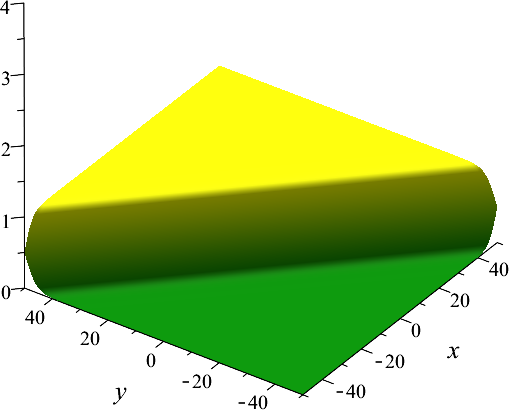
\includegraphics[width=.3\textwidth]{fig/(3+1)JM-1-soliton.png}    
}
\subfigure[2-孤子解 \label{jm:2-soliton}]{
    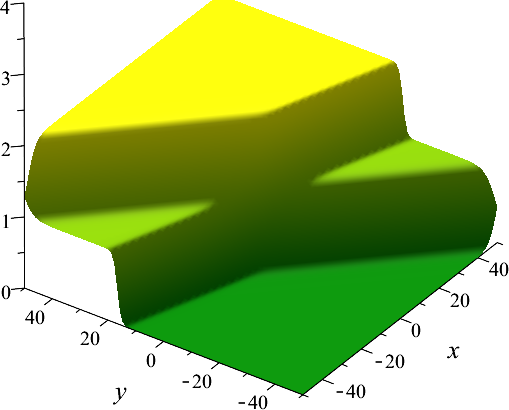
\includegraphics[width=.3\textwidth]{fig/(3+1)JM-2-soliton.png}
}
\subfigure[3-孤子解 \label{jm:3-soliton}]{
    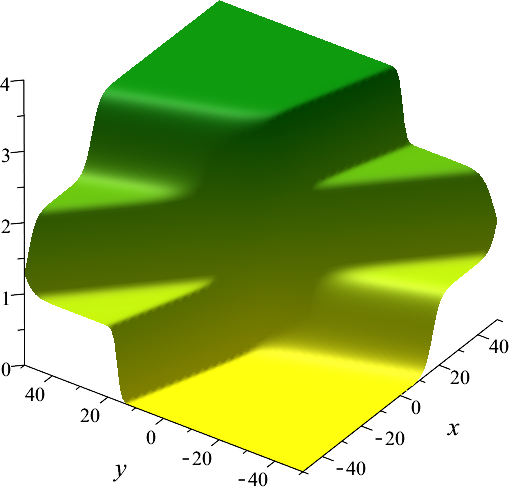
\includegraphics[width=.3\textwidth]{fig/(3+1)JM-3-soliton.png}
}
\subfigure[1-呼吸子解 \label{jm:1-breather}]{
    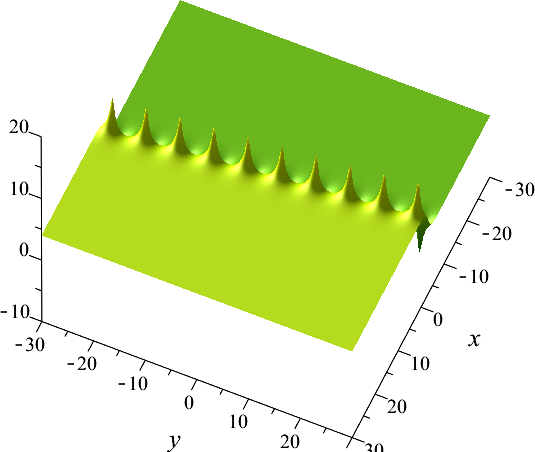
\includegraphics[width=.3\textwidth]{fig/(3+1)JM-1-breather.png}
}
\subfigure[2-呼吸子解 \label{jm:2-breather}]{
    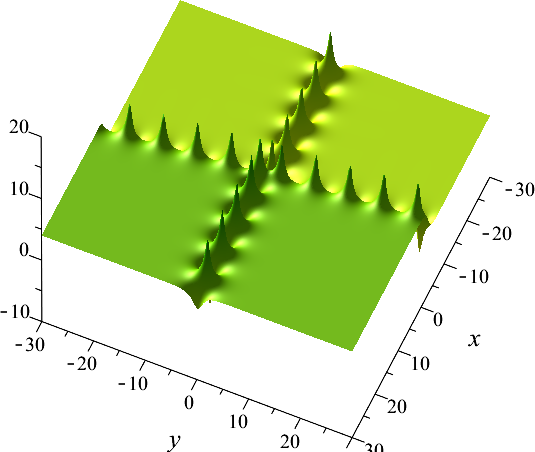
\includegraphics[width=.3\textwidth]{fig/(3+1)JM-2-breather.png}
}
\subfigure[3-呼吸子解 \label{jm:3-breather}]{
    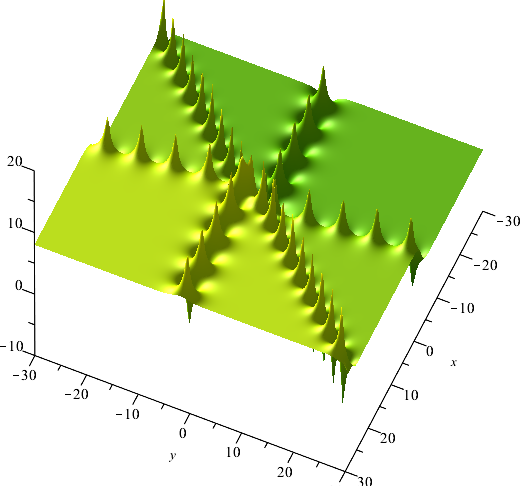
\includegraphics[width=.3\textwidth]{fig/(3+1)JM-3-breather.png}
}
\subfigure[1-lump解 \label{jm:1-lump}]{
    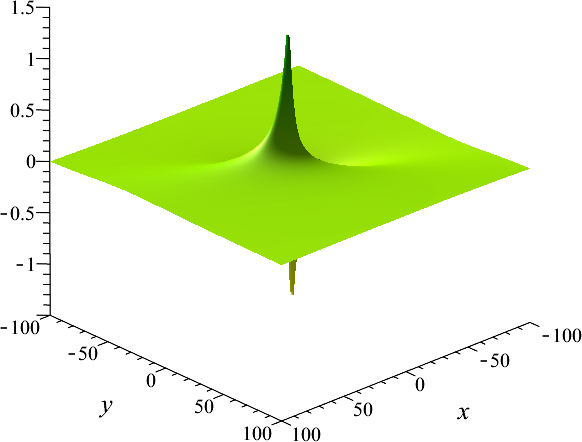
\includegraphics[width=.3\textwidth]{fig/(3+1)JM-1-lump.png}
}
\subfigure[2-lump解 \label{jm:2-lump}]{
    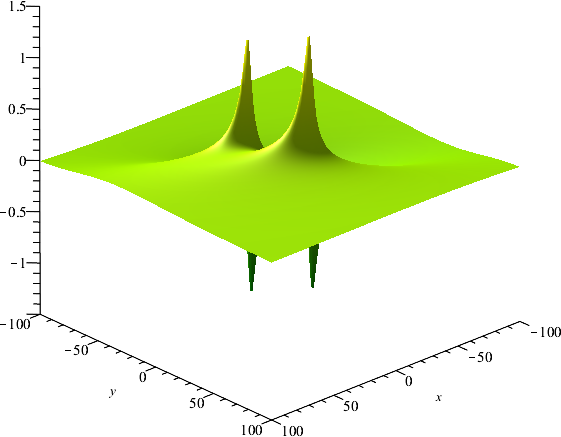
\includegraphics[width=.3\textwidth]{fig/(3+1)JM-2-lump.png}
}
\subfigure[3-lump解 \label{jm:3-lump}]{
    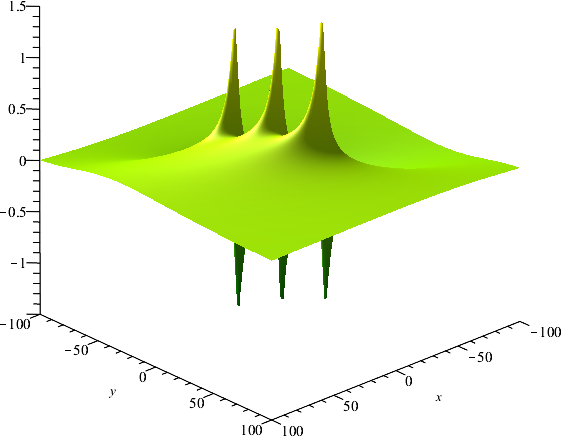
\includegraphics[width=.3\textwidth]{fig/(3+1)JM-3-lump.png}
}
\caption{(3+1)维 JM方程的解}
\label{jm}
\end{figure}

\begin{figure}[p]
\centering
\subfigure[周期波解 \label{jm:1-periodic}]{
    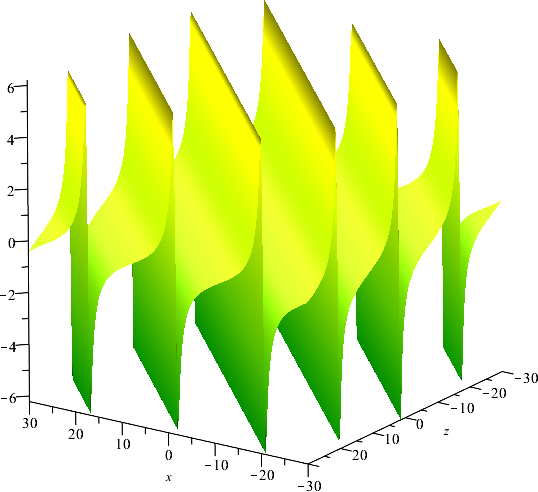
\includegraphics[width=.4\textwidth]{fig/(3+1)JM-1-periodic.png}
}
\subfigure[孤子-呼吸子相互作用解 \label{jm:soliton-breather}]{
    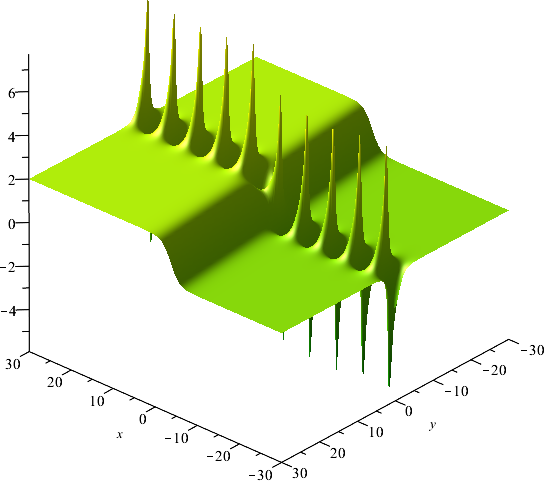
\includegraphics[width=.4\textwidth]{fig/(3+1)JM-soliton-breather.png}
}
\caption{(3+1)维 JM方程的退化解} \label{jmd}
\end{figure}


最终, 基于这些中间结果, 可以按照下述方法分别计算孤子解\D 呼吸子解和lump解:
\begin{compactitem}[\textbullet]
\item 将$\omega$和$h_{i,j}$代入\refeqn{f-soliton-new}可以得到孤子解. \reffig{jm}(a)-(c)分别展示了1-孤子\D 2-孤子和3-孤子解的图像. 
\item 将$\omega$和$h_{i,j}$代入\refeqn{f-breather}可以得到呼吸子解. \reffig{jm}(d)-(f)分别展示了1至3阶呼吸子解的图像.
\item 将$\theta$和$b_{i,j}$代入\refeqn{f-lump-new}可以得到lump解. \reffig{jm}(g)-(i)分别展示了1至3阶lump解的图像.  
\end{compactitem}

有趣的是, 对于1-呼吸子解, 如果关于自变量$x,y$进行作图, 将会得到\reffig{jm:1-breather}; 而关于自变量$x,z$进行作图, 将会得到如\reffig{jm:1-periodic}所示的周期波解. 并且, 对于2-呼吸子解, 若取其中一个呼吸子的参数为实数, 另一个呼吸子的参数仍是复数, 则其图像如\reffig{jm:soliton-breather}所示. 这可以看做是一个扭状孤子和一个呼吸子的相互作用解. 

\reffig{jm}和\reffig{jmd}的作图参数如\reftab{jm-plist}所示.

\begin{table}[htbp]
\centering 
\caption{\reffig{jm}和\reffig{jmd}的作图参数\label{jm-plist}}
\small
\renewcommand{\arraystretch}{1.1}
\begin{tabular}{cp{0.8\textwidth}}
\hline 
\multicolumn{1}{c}{图} & \multicolumn{1}{c}{作图参数} \\ 
\hline 
\ref{jm:1-soliton} & \texttt{{c=0, q=1, t=0, x=-50..50, y=-50..50, z=0, k[1]=1/2, p[1]=1}} \\
\ref{jm:2-soliton} & \texttt{{c=0, q=1, t=0, x=-50..50, y=-50..50, z=0, k[1]=1/2, k[2]=1/2, p[1]=1, p[2]=3}} \\
\ref{jm:3-soliton} & \texttt{{c=0, q=1, t=0, x=-50..50, y=-50..50, z=0, k[1]=1/2, k[2]=1/2, k[3]=1/2, p[1]=1, p[2]=3, p[3]=1/3}} \\
\ref{jm:1-breather} & \texttt{{c=0, q=1, t=0, x=-30..30, y=-30..30, z=0, k[1,IM]=0, k[1,RE]=1, p[1,IM]=1, p[1,RE]=1/10}} \\
\ref{jm:2-breather} & \texttt{{c=0, q=1, t=0, x=-30..30, y=-30..30, z=0, k[1,IM]=0, k[1,RE]=1, k[2,IM]=1, k[2,RE]=0, p[1,IM]=1, p[1,RE]=1/10, p[2,IM]=1, p[2,RE]=1/10}} \\
\ref{jm:3-breather} & \texttt{{c=0, q=1, t=0, x=-30..30, y=-30..30, z=0, k[1,IM]=0, k[1,RE]=1, k[2,IM]=1, k[2,RE]=0, k[3,IM]=1, k[3,RE]=1, p[1,IM]=1, p[1,RE]=1/10, p[2,IM]=1, p[2,RE]=1/10, p[3,IM]=1, p[3,RE]=1/10}} \\
\ref{jm:1-lump} & \texttt{{q=1, t=0, x=-100..100, y=-100..100, z=0, p[1,IM]=1, p[1,RE]=1}} \\
\ref{jm:2-lump} & \texttt{{q=1, t=0, x=-100..100, y=-100..100, z=0, p[1,IM]=1, p[1,RE]=1, p[2,IM]=1, p[2,RE]=6/5}} \\
\ref{jm:3-lump} & \texttt{{q=1, t=0, x=-100..100, y=-100..100, z=0, p[1,IM]=1, p[1,RE]=1, p[2,IM]=1, p[2,RE]=6/5, p[3,IM]=1, p[3,RE]=4/5}} \\
\ref{jm:1-periodic} & \texttt{{c=0, q=1, t=0, x=-30..30, y=0, z=-30..30, k[1,IM]=1/3, k[1,RE]=0, p[1,IM]=1, p[1,RE]=1/10}} \\
\ref{jm:soliton-breather} & \texttt{{c=0, q=1, t=0, x=-30..30, y=-30..30, z=0, k[1,IM]=1, k[1,RE]=0, k[2,IM]=0, k[2,RE]=1, p[1,IM]=1, p[1,RE]=1/10, p[2,IM]=0, p[2,RE]=1/10}} \\

\hline
\end{tabular}
\end{table}

\section{TwSolver软件包的实现与应用}
基于上文描述的算法, 我们在 Maple 中研发了软件 TwSolver. 在本节中, 我们将简要地介绍 TwSolver 的接口. 

在本文中, 我们基于 Maple 的语法来描述软件包的接口. TwSolver 的主要接口是 
\begin{verbatim}
sh:=twsolve(eq,PS,{PL,select_solution});
\end{verbatim}
其中 \verb|{}|中的参数是可选的. 这些参数的意义如下: 
\begin{compactitem}[\textbullet]
\item \cd{eq}表示输入方程, 它需要满足\refeqn{oeq}的形式.
\item \cd{PS}表示\emph{参数下标集合}, 它和$\PS$的意义保持一致. 
\item \cd{PL}是参数列表, 它和$PL$的意义保持一致.
\item \cd{select\_solution}是在多解情况下使用人工选择的参数. 在指定这个参数的情况下, 如果在求解过程中遇到了多解的情况, 程序将会弹出一个对话框让用户选择解的序号. 否则, 程序默认选择第一个解.
\item 返回值\cd{sh}是一个\cd{SolHolder}对象. 它保存了计算的中间结果, 如$\omega,h_{i,j},\theta,b_{i,j}$等. 这些关键参数用于构造孤子解\D 呼吸子解和lump解. 
\end{compactitem}
    
例如, 考虑(2+1)维 BKP方程\CITEbaBKP
\begin{equation}
\begin{split}
0&=u_t+u_{xxxxx}-5u_{xxy}-5\int{u_{yy}\dd{x}}+15u_xu_{xx}\\
&+15uu_{xxx}-15uu_y-15u_x\int{u_y\dd{x}}+45u^2u_x, \label{BKP}
\end{split}
\end{equation}
因为它不满足\refeqn{oeq}的形式, 故不能用\cd{twsolve}直接求解它. 令$v=u_x$, 我们有
\begin{equation}
\begin{split}
0&=v_{tx}+v_{xxxxxx}-5v_{xxxy}-5v_{yy}+15v_{xx}v_{xxx}\\
&+15v_xv_{xxxx}-15v_xv_{xy}-15v_{xx}v_y+45v_x^2v_{xx}. \label{BKP-T}
\end{split}
\end{equation}
该方程可直接被 TwSolver 求解, 调用语句为
\begin{verbatim}
sh:=twsolve(eq,{1,2,3},PL=[k,p,c]); 
\end{verbatim}
其中\cd{eq}是\refeqn{BKP-T}, 而\cd{PL=[k,p,c]}将行波变量指定为$\xi=k(x+py+\omega t)+c$. 如果没有指定\cd{PL}, 则默认$\xi=p_1(x+p_2 y+\omega t)+p_3$. 

事实上, 该方程具有2个不同的TPE:
\begin{equation}
v=\frac{2f_x}{f}\text{~~和~~}v=\frac{4f_x}{f}.
\end{equation}
默认情况下, \cd{select\_solution = false}, 程序会选择$v=2f_x/f$. 而取\cd{select\_solution = true}之后, 我们可以在弹出对话框中任选其中的一个解. 调用语句为
\begin{verbatim}
sh:=twsolve(eq,{1,2,3},PL=[k,p,c],select_solution=true).
\end{verbatim}
在这个例子中, 在对话框中输入1表示选择$v=2f_x/f$. 在这个变换下我们能够求得所有三种类型的解. 但是, 当选择$v=4f_x/f$时, 变换后的方程是不可解的. 类似地, 选项\cd{select\_solution}也能在其它多解的情况下发挥作用.

最终, 该方程的关键参数为
\begin{equation}
\begin{split}
\omega&=-{k}^{4}+5\,{k}^{2}p+5\,{p}^{2}, \\ 
h_{i,j}&=[{k_{{i}}}^{4}-3\,{k_{{i}}}^{3}k_{{j}}+ \left( 4\,{k_{{j}}}^{2}-2\,p_{{i}}-p_{{j}} \right) {k_{{i}}}^{2}-3\,k_{{j}} \left( {k_{{j}}}^{2}-p_{{i}}-p_{{j}} \right) k_{{i}}+{k_{{j}}}^{4}\\
&+\left( -p_{{i}}-2\,p_{{j}}\right) {k_{{j}}}^{2}+ \left( p_{{i}}-p_{{j}} \right) ^{2}]/[{k_{{i}}}^{4}+3\,{k_{{i}}}^{3}k_{{j}}+ \left( 4\,{k_{{j}}}^{2}-2\,p_{{i}}-p_{{j}} \right) {k_{{i}}}^{2}\\
&+3\,k_{{j}} \left( {k_{{j}}}^{2}-p_{{i}}-p_{{j}} \right) k_{{i}}+{k_{{j}}}^{4}+ \left( -p_{{i}}-2\,p_{{j}}\right) {k_{{j}}}^{2}+ \left( p_{{i}}-p_{{j}} \right) ^{2}].
\end{split}
\end{equation}

关于解的一系列操作都可以基于返回对象\cd{sh}完成.  它提供了如下接口: 
\begin{compactitem}[\textbullet]
\item \cd{sh:-get\_sol(type,m)}能够自动推导类型为\cd{type}的$m$阶解. 
\item \verb|sh:-verify_sol(type,m,{s,rnd_assign,method})|用于验证求得的解是否满足原方程. 这里,
\begin{compactitem}[- ]
\item \cd{s}是参数赋值的集合.
\item 如果指定选项\cd{rnd\_assign}, 程序将对\cd{s}中没有赋值的剩余参数进行随机赋值.
\item \cd{method}用于指定验证解的方法. 我们将在下文中具体介绍这个参数. 
\end{compactitem}
\item \verb|sh:-plot_sol(sol,s)|用于绘制解. 其中
\begin{compactitem}[- ]
\item \cd{sol} 表示一个解. 
\item \cd{s} 是一个参数赋值的集合. 在作图时, 所有参数都应该被赋值, 并且需要指定各个自变量的取值范围.
\end{compactitem}
\end{compactitem}

对于上面的例子, \cd{sh:-get\_sol(soliton,1)}将会输出(2+1)维 BKP-T 方程的1-孤子解, 即 
\begin{equation}
v=2\,{\frac {k_{{1}}{{\rm e}^{k_{{1}} \left(  \left( -{k_{{1}}}^{4}+5\,{
k_{{1}}}^{2}p_{{1}}+5\,{p_{{1}}}^{2} \right) t+p_{{1}}y+x \right)+c_1 }}}{
1+{{\rm e}^{k_{{1}} \left(  \left( -{k_{{1}}}^{4}+5\,{k_{{1}}}^{2}p_{{
1}}+5\,{p_{{1}}}^{2} \right) t+p_{{1}}y+x \right)+c_1 }}}}.
\end{equation}

因为验证解的时间要大于求解的时间, 为了用户的方便, 我们将求解和验证两个过程拆分开来. 在我们的算法中, 3阶及以上的孤子解和2阶及以上的呼吸子解和lump解可能不满足原方程. 因此, 我们需要利用\cd{sh:-verify\_sol(type,m)}来验证解. 因为对参数赋值后能够极大地提高验证的速度, 我们可以对参数进行人工赋值或者自动赋值. 例如, \cd{sh:-verify\_sol(soliton,3,rnd\_assign)} 表示对求得的3-孤子解在随机赋值的参数条件下进行验证, 大概耗时0.06秒. 然而, \cd{sh:-verify\_sol(soliton,3,$\{k_1=1,k_2=2,k_3=3\}$)}仅对部分参数进行了人工赋值, 它的运行时间约为10秒. 所以, 参数赋值能够极大地提高验证解的速度. 

为了进一步提高验证解的速度, 我们考虑了三种不同的验证方法: 
\begin{compactenum}[method-1:]
\item 将解代入变换后的方程, 验证指数项的各项系数是否为零.
\item 将解代入变换后的方程, 验证方程左端是否为零.
\item 将解代入原方程, 验证方程左端是否为零.
\end{compactenum}
\mk{我们会在\refsec{ch02exp}的实验中说明 method-1是最快的方法.}{那个表远着呢, 这么早提似乎不好}

在绘制解的函数中, 其参数和求解以及验证函数的参数有所不同. 如果要直接对得到的$m$-type解进行作图, 可以调用\cd{sh:-plot\_sol([type,m],s)}. 例如, 
\begin{verbatim}
sh:-plot_sol(
    [soliton,1],
    {k[1]=1/4,p[1]=1/5,c[1]=0,t=0,x=-50..50,y=-50..50}
)
\end{verbatim}
可绘制(2+1)维 BKP-T方程的1-孤子解. 该解如\reffig{bkp:1-soliton-t}所示, 是一个扭状孤子.

因为$u=v_x$, 如果要绘制(2+1)维 BKP方程的1-孤子解, 可以用 
\begin{verbatim}
sh:-plot_sol(
    diff(sh:-get_sol(soliton,1),x),
    {k[1]=1/4,p[1]=1/5,c[1]=0,t=0,x=-50..50,y=-50..50}
)
\end{verbatim} 
进行绘制. 该解如\reffig{bkp:1-soliton}所示, 是一个钟状孤子.

此外, \cd{sh:-plot\_sol}还能接受\cd{plot3d}的参数来改变绘制结果的外形. 例如, 
\begin{verbatim}
sh:-plot_sol(
    diff(sh:-get_sol(soliton,2),x),
    {k[1]=1/4,p[1]=1/5,k[2]=1/4,p[2]=-2,
    c[1]=0,c[2]=5,x=-50..50,y=-50..50,t=0},
    grid=[400,400],style=surface,
    colorscheme=["zgradient",["Green","Yellow"]]
)
\end{verbatim} 
可绘制(2+1)维 BKP方程的2-孤子解. 其图像如\reffig{bkp:2-soliton}所示, 它是由两个钟状孤子相互作用而成的, 我们通过设置\cd{plot3d}的参数改变了它的外形.

\begin{figure}[H]
\centering
\subfigure[BKP-T方程的1-孤子解 \label{bkp:1-soliton-t}]{
    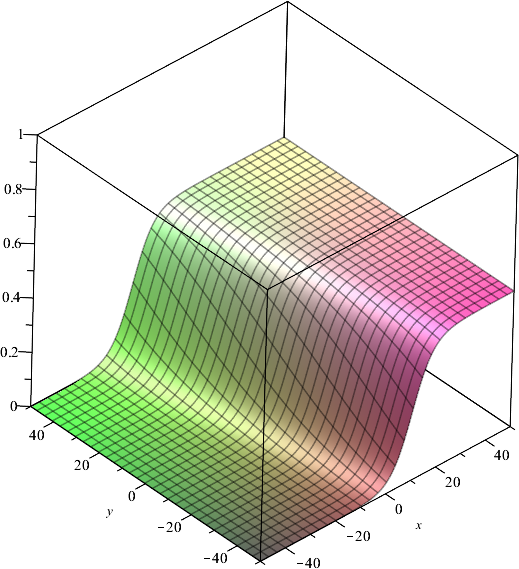
\includegraphics[width=.3\textwidth]{fig/(2+1)BKP-T-1-soliton.png}
}
\subfigure[BKP方程的1-孤子解 \label{bkp:1-soliton}]{
    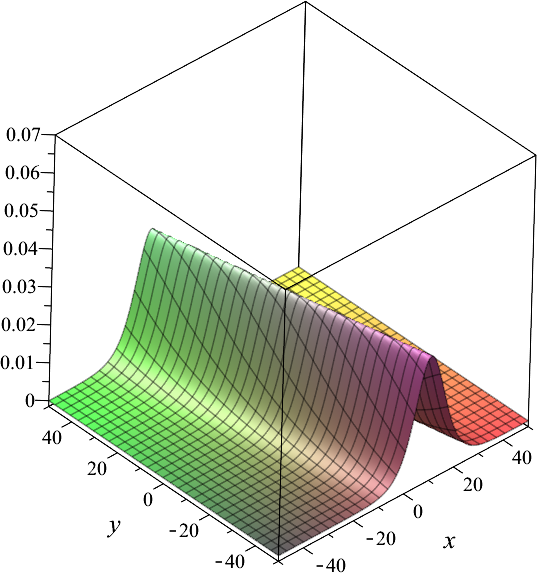
\includegraphics[width=.3\textwidth]{fig/(2+1)BKP-1-soliton.png}
}
\subfigure[BKP方程的2-孤子解 \label{bkp:2-soliton}]{
    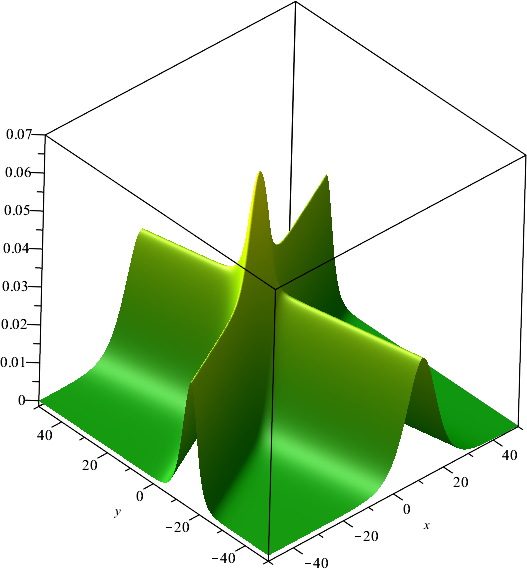
\includegraphics[width=.3\textwidth]{fig/(2+1)BKP-2-soliton.png}
}
\caption{(2+1)维 BKP/BKP-T方程的孤子解}\label{bkp}
\end{figure}

\section{实验与分析}\label{ch02exp}
$\PS$在我们的算法中起着非常重要的作用, 我们选择了一些具有代表性的方程, 在不同的$\PS$取值下对它们进行求解, 来探索$\PS$和方程之间的关系. 实验结果如\reftab{verify}所示. 在\reftab{verify}中, 第一列表示方程名. 方程名的后缀`-T'表示经过变换的方程, 后缀`-G'表示经过推广的方程. 第二列是$\PS$取值的简写. 例如, `12' 表示$\PS=\{1,2\}$. 我们的测试忽略了行波变量中的常数项, 因为它不会对实验结果造成影响. 

\begin{table}[htbp]
\centering 
\caption{TwSolver中一些方程的解的验证结果} \label{verify}
\small
\begin{tabular}{lrcccc}
\hline
\multicolumn{1}{c}{方程名}&\multicolumn{1}{c}{$\PS$} &3-孤子 &2-呼吸子 &2-lump &无解原因\\
\hline
(1+1) KdV &1 &\VTRUE &\VTRUE &- &err-2\\
(2+1) BKP-T &1 &\VTRUE &\VTRUE &- &err-2\\
(2+1) BKP-T &12 &\VTRUE &\VTRUE &\VTRUE &\\
(2+1) CBS &1 &\VTRUE &\VTRUE &- &err-2\\
(2+1) CBS &12 &\VTRUE &\VTRUE &- &err-3\\
(2+1) CBS-G &1 &\VTRUE &\VTRUE &- &err-2\\
(2+1) CBS-G &12 &\VFALSE &\VFALSE &\VFALSE &\\
(2+1) KP &1 &\VTRUE &\VTRUE &- &err-2\\
(2+1) KP &12 &\VTRUE &\VTRUE &\VTRUE &\\
(2+1) SK &1 &\VTRUE &\VTRUE &- &err-2\\
(2+1) SK &12 &\VTRUE &\VTRUE &\VTRUE &\\
(3+1) BKP &1 &\VTRUE &\VTRUE &- &err-2\\
(3+1) BKP &12 &\VTRUE &\VTRUE &\VTRUE &\\
(3+1) BKP &13 &\VTRUE &\VTRUE &\VTRUE &\\
(3+1) BKP &123 &\VFALSE &\VFALSE &\VFALSE &\\
(3+1) CBS &1 &\VTRUE &\VTRUE &- &err-2\\
(3+1) CBS &12 &\VTRUE &\VTRUE &- &err-3\\
(3+1) CBS &13 &\VTRUE &\VTRUE &- &err-3\\
(3+1) CBS &123 &\VTRUE &\VTRUE &- &err-3\\
(3+1) JM &1 &\VTRUE &\VTRUE &- &err-2\\
(3+1) JM &12 &\VTRUE &\VTRUE &\VTRUE &\\
(3+1) JM &13 &\VTRUE &\VTRUE &- &err-3\\
(3+1) JM &123 &\VFALSE &\VFALSE &\VFALSE &\\
(3+1) KP &1 &\VTRUE &\VTRUE &- &err-2\\
(3+1) KP &12 &\VTRUE &\VTRUE &\VTRUE &\\
(3+1) KP &13 &\VTRUE &\VTRUE &\VTRUE &\\
(3+1) KP &123 &\VFALSE &\VFALSE &\VFALSE &\\
(3+1) NEE-T &1 &\VTRUE &\VTRUE &- &err-2\\
(3+1) NEE-T &12 &\VTRUE &\VTRUE &\VTRUE &\\
(3+1) NEE-T &13 &\VTRUE &\VTRUE &- &err-3\\
(3+1) NEE-T &123 &\VFALSE &\VFALSE &\VFALSE &\\
(3+1) YTSF &1 &\VTRUE &\VTRUE &- &err-2\\
(3+1) YTSF &12 &\VTRUE &\VTRUE &\VTRUE &\\
(3+1) YTSF &13 &\VTRUE &\VTRUE &- &err-3\\
(3+1) YTSF &123 &- &- &- &err-1\\
(4+1) Fokas-T &1 &\VTRUE &\VTRUE &- &err-2\\
(4+1) Fokas-T &12 &\VTRUE &\VTRUE &- &err-3\\
(4+1) Fokas-T &13 &\VTRUE &\VTRUE &- &err-3\\
(4+1) Fokas-T &123 &\VFALSE &\VFALSE &\VFALSE &\\
(4+1) Fokas-T-2 &1 &\VTRUE &\VTRUE &- &err-2\\
(4+1) Fokas-T-2 &12 &\VTRUE &\VTRUE &\VTRUE &\\
\hline
\multicolumn{6}{l}{\pbox{0.6\textwidth}{
{\tiny ~}\\
注: err-1表示$h_{i,j}$ 无解, err-2表示lump解需要$\{1\}\subsetneq \PS$, err-3表示0作为除数. 表中出现的方程如果未出现在本章中, 则其表达式在\reftab{eqs}中.
}}
\end{tabular}
\end{table}

\begin{table}[htbp]
\centering
\caption{TwSolver中测试方程的表达式列表}\label{eqs}
\renewcommand{\arraystretch}{1.2}
\begin{tabular}{lp{0.7\textwidth}}
\hline
\multicolumn{1}{c}{方程名} & \multicolumn{1}{c}{表达式} \\
\hline
(2+1) SK\CITEbaSK & $5\,{u_{{x}}}^{2}u_{{{\it xx}}}+5\,u_{{x}}u_{{{\it xxxx}}}+5\,u_{{x}}u_{{{\it xy}}}+5\,u_{{{\it xx}}}u_{{{\it xxx}}}+5\,u_{{{\it xx}}}u_{{y}}-u_{{{\it tx}}}+u_{{{\it xxxxxx}}}+5\,u_{{{\it xxxy}}}-5\,u_{{{\it yy}}}=0$.\\
(2+1) KP\CITEbaKP & $\alpha\,u_{{{\it yy}}}+6\,uu_{{{\it xx}}}+6\,{u_{{x}}}^{2}+u_{{{\it tx}}}+u_{{{\it xxxx}}}=0$.\\
(2+1) CBS\CITEbaCBS & $4\,u_{{x}}u_{{{\it xy}}}+2\,u_{{{\it xx}}}u_{{y}}+u_{{{\it tx}}}+u_{{{\it xxxy}}}=0$.\\
(2+1) CBS-G\CITEbaCBSG & $\alpha\,u_{{{\it xy}}}+\beta\,u_{{{\it yy}}}+3\,u_{{x}}u_{{{\it xy}}}+3\,u_{{{\it xx}}}u_{{y}}+u_{{{\it tx}}}+u_{{{\it xxxy}}}=0$.\\
(3+1) CBS\CITEcaCBS & $4\,u_{{x}}u_{{{\it xy}}}+4\,u_{{x}}u_{{{\it xz}}}+2\,u_{{{\it xx}}}u_{{y}}+2\,u_{{{\it xx}}}u_{{z}}+u_{{{\it tx}}}+u_{{{\it xxxy}}}+u_{{{\it xxxz}}}=0$.\\
(3+1) BKP\CITEcaBKP & $-3\,u_{{x}}u_{{{\it xy}}}-3\,u_{{{\it xx}}}u_{{y}}+u_{{{\it ty}}}+3\,u_{{{\it xx}}}-u_{{{\it xxxy}}}+3\,u_{{{\it zz}}}=0$.\\
(3+1) KP\CITEcaKP & $-6\,uu_{{{\it xx}}}-6\,{u_{{x}}}^{2}+u_{{{\it tx}}}+u_{{{\it xxxx}}}+3\,u_{{{\it yy}}}+3\,u_{{{\it zz}}}=0$.\\
(3+1) NEE\CITEcaNEE & $3\,u_{{{\it xz}}}-2\,u_{{{\it ty}}}-u_{{{\it xxxy}}}+4\,u_{{x}}u_{{y}}+2\,uu_{{{\it xy}}}+2\,u_{{{\it xx}}}\int \!u_{{y}}\,{\rm d}x=0$.\\
(3+1) NEE-T\CITEcaNEET & $2\,v_{{x}}v_{{{\it xxy}}}+4\,v_{{{\it xx}}}v_{{{\it xy}}}+2\,v_{{{\it xxx}}}v_{{y}}-2\,v_{{{\it txy}}}-v_{{{\it xxxxy}}}+3\,v_{{{\it xxz}}}=0$.\\
(3+1) YTSF\CITEcaYTSF & $3\,\alpha\,u_{{{\it yy}}}+4\,u_{{x}}u_{{{\it xz}}}+2\,u_{{{\it xx}}}u_{{z}}-4\,u_{{{\it tx}}}+u_{{{\it xxxz}}}=0$.\\

\hline
\end{tabular}
\end{table}

因为1-孤子和2-孤子是通过待定系数法直接求解的, 所以它们必然满足原方程. 而1-呼吸子和1-lump是由2-孤子解生成的, 也不需要验证. 因此, 我们在实验中验证3-孤子解\D 2-呼吸子解和2-lump解. 表中`\VTRUE'表示得到的解是\TrueSol{}, `\VFALSE'表示得到的解是\FalseSol{}. 此外, `-'表示由我们的方法不能得到解, 并且无解的原因会在最后一列给出. 

从\reftab{verify}中可以看出, 所有的方程在$\PS=\{1\}$时都能够得到满足原方程的孤子和呼吸子解. 

除了(2+1)维 CBS-G方程以外的大多数的(2+1)维的方程在$\PS= \ALLP$时如果有解, 则解是满足原方程的. \red{此外, 除(2+1)维 CBS方程和(2+1)维 GBS-G 方程以外的(2+1)维方程都有 lump 解.}

除了(3+1)维 CBS方程以外的所有(3+1)维方程在$\PS= \ALLP$时不能得到\TrueSol{}. 但是, 这些方程在$\PS=\{1,2\}$或$\PS=\{1,3\}$时都能得到\TrueSol{}. 事实上, 这些方程在$(p_i,q_i)~(i=1,2,\cdots)$线性相关时能够得到\TrueSol{}.

因此, 随着维数的增加, $\PS$对于获得\TrueSol{}的作用越来越大. 除了限定$\PS$之外, 方程降维也是将我们的方法推广到高维的重要手段. (4+1)维 Fokas 方程\CITEdaFokas{}就是一个典型的例子. 它的表达式为
\begin{equation}
    u_{tx}-\frac{1}{4}u_{xxxy}+\frac{1}{4}u_{xyyy}+3u_xu_y+3uu_{xy}-\frac{3}{2}u_{wz}=0. \label{Fokas}
\end{equation}
当$\PS=\{1,3,4\}$, 该方程能够被我们的算法直接求解. 对应的TPE为
\begin{equation}
u={\frac {{f_{{x}}}^{2}-{f_{{y}}}^{2}}{{f}^{2}}}+{\frac { \left( -5\,f_{
{{ xx}}}+f_{{{ yy}}} \right) {f_{{x}}}^{2}+8\,f_{{x}}f_{{y}}f_{{
{ xy}}}+{f_{{y}}}^{2} \left( f_{{{ xx}}}-5\,f_{{{ yy}}}
\right) }{5f(f_x^2-f_y^2)}}.
\end{equation}
但是计算对应的$\omega$和$h_{i,j}$则比较慢. 在我们的实验中, 该方程的求解大约耗时90秒, 而验证解的时间则很长. 

因为上述TPE是关于$f,f_x$和$f_y$的函数, 我们决定取行波变换$\xi=ax+by$进行降维. 可以得到
\begin{equation}
    au_{t\xi}-\frac{a^3b}{4}u_{\xi\xi\xi\xi}+\frac{ab^3}{4}u_{\xi\xi\xi\xi}+3abu_{\xi}^2+3abuu_{\xi\xi}-\frac{3}{2}u_{wz}=0.  \label{Fokas-T}
\end{equation}
这个方程在\reftab{verify}中被称为是\mk{(4+1) Fokas-T方程}{其实维数是(3+1)的, 但是名字是这个, 所以不加维字了, 或者统一改为 (3+1) Fokas 和 (2+1) Fokas ??}. 将原方程降为(3+1)维方程之后, 对应的TPE变为
\begin{equation}
    u=(a^2-b^2)\sbrace{\frac{f_{\xi}^2}{f^2}-\frac{f_{\xi\xi}}{f}}.
\end{equation}
取$\PS=\{1,2,3\}$, 我们得到
\begin{equation}
\begin{split}
    \omega&={\frac {{a}^{3}b{k}^{2}-a{b}^{3}{k}^{2}+6\,pq}{4a}}, \\
    h_{{i,j}}&={\frac {b \left( k_{{i}}-k_{{j}} \right) ^{2}{a}^{3}-{b}^{3}
    \left( k_{{i}}-k_{{j}} \right) ^{2}a-2\, \left( q_{{i}}-q_{{j}}
    \right)  \left( p_{{i}}-p_{{j}} \right) }{b \left( k_{{i}}+k_{{j}}
    \right) ^{2}{a}^{3}-{b}^{3} \left( k_{{i}}+k_{{j}} \right) ^{2}a-2\,
    \left( q_{{i}}-q_{{j}} \right)  \left( p_{{i}}-p_{{j}} \right) }}.
\end{split}
\end{equation}
从\reftab{verify}中可以看出, 当$\PS=\{1,2,3\}$时, 方程无\TrueSol{}. 但是当$\PS=\{1,2\}$或$\PS=\{1,3\}$时, 方程有\TrueSol{}. 事实上, 和大多数(3+1)维方程一样, 当$(p_i,q_i)~(i=1,2,\cdots)$线性相关时, \refeqnn{Fokas-T}有\TrueSol{}.

基于上述发现, 我们对\red{(4+1) Fokas-T方程}取行波变换$\eta=cw+dz$得到
\begin{equation}
    au_{t\xi}-\frac{a^3b}{4}u_{\xi\xi\xi\xi}+\frac{ab^3}{4}u_{\xi\xi\xi\xi}+3abu_{\xi}^2+3abuu_{\xi\xi}-\frac{3cd}{2}u_{\eta\eta}=0.  \label{Fokas-T-2}
\end{equation}
该方程在\reftab{verify}中被记作\red{(4+1) Fokas-T-2}. 该方程的关键参数是
\begin{equation}
\begin{split}
    \omega&={\frac {{a}^{3}b{k}^{2}-a{b}^{3}{k}^{2}+6\,cd{p}^{2}}{4a}}, \\ 
    h_{{i,j}}&={\frac {b \left( k_{{i}}-k_{{j}} \right) ^{2}{a}^{3}-{b}^{3}
    \left( k_{{i}}-k_{{j}} \right) ^{2}a-2\,cd \left( p_{{i}}-p_{{j}}
    \right) ^{2}}{b \left( k_{{i}}+k_{{j}} \right) ^{2}{a}^{3}-{b}^{3}
    \left( k_{{i}}+k_{{j}} \right) ^{2}a-2\,cd \left( p_{{i}}-p_{{j}}
    \right) ^{2}}}.
\end{split}
\end{equation}
从\reftab{verify}中可以看出, 该方程在$\PS=\{1,2\}$时有\TrueSol{}.

\reftab{verify}中所有例子的运行时间如\reftab{runtime}所示. 从\reftab{runtime}中可以看出, method-1是最快的. 这是因为 method-1 在验证2-呼吸子解时存在显著优势, 而2-呼吸子的验证又是耗时最长的. 因此, \cd{sh:-verify\_sol}的默认选项是\cd{method=1}. 

\begin{table}[htbp]
\centering 
\caption{TwSolver 中验证解的运行时间} \label{runtime}
\begin{tabular}{c|ccc|c}
\hline
time(h) &method-1 &method-2 &method-3 &sum\\
\hline
solve &0.002 &0.002 &0.002 &0.005\\
3-soliton &0.002 &0.002 &0.016 &0.020\\
2-breather &0.212 &0.949 &1.551 &2.713\\
2-lump &0.022 &0.022 &0.033 &0.077\\
\hline
sum &0.238 &0.975 &1.602 &2.815\\
\hline
\end{tabular}
\end{table}

\section{小结}
在本章中, 我们开发了求解 NLEE 三种波解的软件包 TwSolver, 该软件包对解的计算\D 验证和作图都提供了简单方便的接口. TwSolver 首先利用 \Painleve{}展开法确定变换, 然后通过简单 Hirota 方法构造孤子解. 获得孤子解之后, 通过共轭参数法得到呼吸子解, 基于长极限法计算 lump 解.  本文的主要工作在于: 
\begin{compactenum}[(1)]
\item 首次对\Painleve{}展开法中待定函数的求解方法进行了分析讨论, 提出了一个递归求解算法. 
\item 提出了\emph{参数下标集合}$\PS$来描述参数的约束条件, 将$n$孤子解的公式推广到不可积方程, 为获得不可积方程的真解提供了有效的途径.
\item 首次推导了一般情况下lump解生成公式中关键参数的计算方法.
\item 为了优化编程实现. 重写了孤子解和lump解的生成公式, 并给出了计算lump解生成公式的对应算法.
\end{compactenum}

同时, 文中的实验和例子表明, 随着方程维数的增加, 方程不可积的可能性越来越大. 为了得到高阶方程的真解, 本文总结了以下技巧:
\begin{compactenum}[(1)]
\item 选择合适的\emph{参数下标集合}($\PS\subsetneq  \ALLP$). 
\item 考虑对参数添加线性相关的约束.
\item 基于行波变换对方程进行降维.
\end{compactenum}

本章的研究成果已投到 Computer Physics Communications 上, 目前正在审稿中. 
